\documentclass[lang=cn,11pt,a4paper,chinesefont=founder]{elegantpaper}
\usepackage{indentfirst} 
\usepackage{graphicx} 
\usepackage{subfigure}
\usepackage{ragged2e}
\usepackage{lmodern}
\usepackage{color}

\setmonofont{Consolas}

\title{Buceros: 一个简单的RISC-V SOC}
\author{张政镒 \\ 20300750021 \and 李少群 \\ 20300750018 \and 王彬 \\ 20300750019}
\institute{\href{https://github.com/0xtaruhi/Buceros}{Github项目链接}}
\date{\zhtoday}

\begin{document}

\maketitle
\begin{figure}[h]
    \centering
    
\includegraphics[scale=0.1]{buceros}
\end{figure}
\begin{abstract}
    本文介绍了Buceros团队制作的简单的RISC-V SOC, 以五级流水线的操作, 可以实现70MHz以上的时钟频率, 较之于网上的RISC-V 代码有了更多精进改善之处, 从而更好的节省了资源, 提高了运行速度. 
    \keywords{中央处理器, RISC-V指令集, SOC}
\end{abstract}


\section{概述}
\begin{figure}[h]
    \centering
    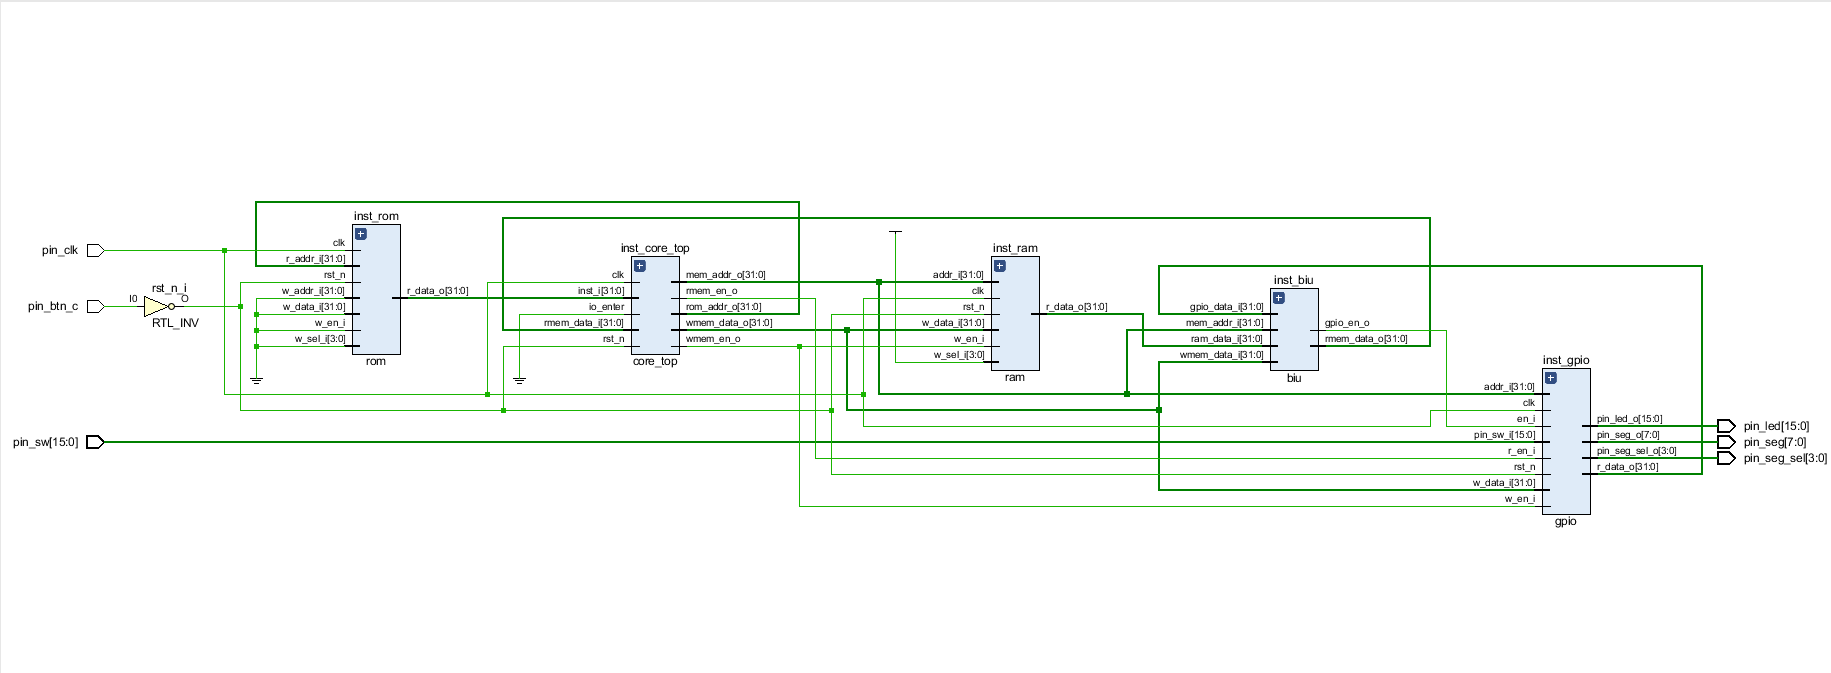
\includegraphics[scale=0.4]{总结构图}
    \caption{总结构图}
\end{figure}
\subsection{core\_top核心模块}
\begin{figure}[h]
    \centering
    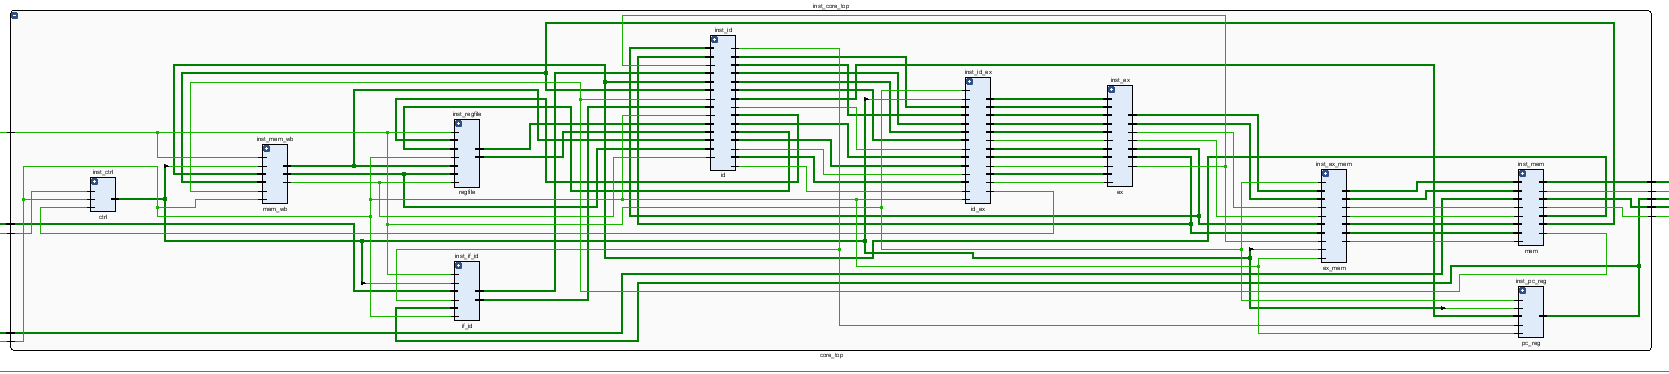
\includegraphics[scale=0.5]{coretop}
\end{figure}
本CPU按照取指(IF), 译码(ID), 执行(EX), 访存(MEM), 回写(WB)的顺序设计五级流水线, 这五者加上ctrl模块及各级寄存器组构成了core\_top模块, 实现了CPU的核心功能, 实现了对RV32I指令集的译码、执行
(不包括ecall和ebreak指令), 实现了本次实验的需求. 
\subsection{RV32I指令集}
与大多数指令集相比, RISC-V指令集可以自由地用于任何目的, 允许任何人设计、制造和销售RISC-V芯片和软件. 虽然这不是第一个开源指令集, 但它具有重要意义, 
因为其设计使其适用于现代计算设备(如仓库规模云计算机、高端移动电话和微小嵌入式系统). 设计者考虑到了这些用途中的性能与功率效率. 
该指令集还具有众多支持的软件, 这解决了新指令集通常的弱点. 

%   \section*{RISC-V Instruction Set}

\subsection*{Core Instruction Formats}
\small
\begin{center}
\begin{tabular}
{p{0in}p{0.4in}p{0.05in}p{0.05in}p{0.05in}p{0.05in}p{0.4in}p{0.6in}p{0.4in}p{0.6in}p{0.7in}l}
&
\multicolumn{1}{l}{\instbit{31}} &
\multicolumn{1}{r}{\instbit{27}} &
\instbit{26} &
\instbit{25} &
\multicolumn{1}{l}{\instbit{24}} &
\multicolumn{1}{r}{\instbit{20}} &
\instbitrange{19}{15} &
\instbitrange{14}{12} &
\instbitrange{11}{7} &
\instbitrange{6}{0} \\
\cline{2-11}

&
\multicolumn{4}{|c|}{funct7} &
\multicolumn{2}{c|}{rs2} &
\multicolumn{1}{c|}{rs1} &
\multicolumn{1}{c|}{funct3} &
\multicolumn{1}{c|}{rd} &
\multicolumn{1}{c|}{opcode} & R-type \\
\cline{2-11}

&
\multicolumn{6}{|c|}{imm[11:0]} &
\multicolumn{1}{c|}{rs1} &
\multicolumn{1}{c|}{funct3} &
\multicolumn{1}{c|}{rd} &
\multicolumn{1}{c|}{opcode} & I-type \\
\cline{2-11}

&
\multicolumn{4}{|c|}{imm[11:5]} &
\multicolumn{2}{c|}{rs2} &
\multicolumn{1}{c|}{rs1} &
\multicolumn{1}{c|}{funct3} &
\multicolumn{1}{c|}{imm[4:0]} &
\multicolumn{1}{c|}{opcode} & S-type \\
\cline{2-11}

&
\multicolumn{4}{|c|}{imm[12$\vert$10:5]} &
\multicolumn{2}{c|}{rs2} &
\multicolumn{1}{c|}{rs1} &
\multicolumn{1}{c|}{funct3} &
\multicolumn{1}{c|}{imm[4:1$\vert$11]} &
\multicolumn{1}{c|}{opcode} & B-type \\
\cline{2-11}

&
\multicolumn{8}{|c|}{imm[31:12]} &
\multicolumn{1}{c|}{rd} &
\multicolumn{1}{c|}{opcode} & U-type \\
\cline{2-11}

&
\multicolumn{8}{|c|}{imm[20$\vert$10:1$\vert$11$\vert$19:12]} &
\multicolumn{1}{c|}{rd} &
\multicolumn{1}{c|}{opcode} & J-type \\
\cline{2-11}
\end{tabular}
\end{center}

\subsection*{RV32I Base Integer Instructions}

\begin{tabular}
{T | l | c | T | T | T | T | l} \hline
\rm Inst & Name                    & FMT & \rm Opcode & \rm funct3 & \rm funct7 & \rm Description (C)          & Note \\ \hline
add      & ADD                     & R   & 0110011    & 0x0    & 0x00   & rd = rs1 + rs2               & \\
sub      & SUB                     & R   & 0110011    & 0x0    & 0x20   & rd = rs1 - rs2               & \\
xor      & XOR                     & R   & 0110011    & 0x4    & 0x00   & rd = rs1 \^{} rs2            & \\
or       & OR                      & R   & 0110011    & 0x6    & 0x00   & rd = rs1 | rs2               & \\
and      & AND                     & R   & 0110011    & 0x7    & 0x00   & rd = rs1 \& rs2              & \\
sll      & Shift Left Logical      & R   & 0110011    & 0x1    & 0x00   & rd = rs1 \verb|<<| rs2       & \\
srl      & Shift Right Logical     & R   & 0110011    & 0x5    & 0x00   & rd = rs1 \verb|>>| rs2       & \\
sra      & Shift Right Arith*      & R   & 0110011    & 0x5    & 0x20   & rd = rs1 \verb|>>| rs2       & msb-extends \\
slt      & Set Less Than           & R   & 0110011    & 0x2    & 0x00   & rd = (rs1 < rs2)?1:0         & \\
sltu     & Set Less Than (U)       & R   & 0110011    & 0x3    & 0x00   & rd = (rs1 < rs2)?1:0         & zero-extends \\ \hline
addi     & ADD Immediate           & I   & 0010011    & 0x0    &        & rd = rs1 + imm               & \\
xori     & XOR Immediate           & I   & 0010011    & 0x4    &        & rd = rs1 \^{} imm            & \\
ori      & OR Immediate            & I   & 0010011    & 0x6    &        & rd = rs1 | imm               & \\
andi     & AND Immediate           & I   & 0010011    & 0x7    &        & rd = rs1 \& imm              & \\
slli     & Shift Left Logical Imm  & I   & 0010011    & 0x1    & imm[5:11]=0x00 & rd = rs1 \verb|<<| imm[0:4]  & \\
srli     & Shift Right Logical Imm & I   & 0010011    & 0x5    & imm[5:11]=0x00 & rd = rs1 \verb|>>| imm[0:4]  & \\
srai     & Shift Right Arith Imm   & I   & 0010011    & 0x5    & imm[5:11]=0x20 & rd = rs1 \verb|>>| imm[0:4]  & msb-extends \\
slti     & Set Less Than Imm       & I   & 0010011    & 0x2    &        & rd = (rs1 < imm)?1:0         & \\
sltiu    & Set Less Than Imm (U)   & I   & 0010011    & 0x3    &        & rd = (rs1 < imm)?1:0         & zero-extends \\ \hline
lb       & Load Byte               & I   & 0000011    & 0x0    &        & rd = M[rs1+imm][0:7]         & \\
lh       & Load Half               & I   & 0000011    & 0x1    &        & rd = M[rs1+imm][0:15]        & \\
lw       & Load Word               & I   & 0000011    & 0x2    &        & rd = M[rs1+imm][0:31]        & \\
lbu      & Load Byte (U)           & I   & 0000011    & 0x4    &        & rd = M[rs1+imm][0:7]         & zero-extends \\
lhu      & Load Half (U)           & I   & 0000011    & 0x5    &        & rd = M[rs1+imm][0:15]        & zero-extends \\ \hline
sb       & Store Byte              & S   & 0100011    & 0x0    &        & M[rs1+imm][0:7]  = rs2[0:7]  & \\
sh       & Store Half              & S   & 0100011    & 0x1    &        & M[rs1+imm][0:15] = rs2[0:15] & \\
sw       & Store Word              & S   & 0100011    & 0x2    &        & M[rs1+imm][0:31] = rs2[0:31] & \\ \hline
beq      & Branch ==               & B   & 1100011    & 0x0    &        & if(rs1 == rs2) PC += imm     & \\
bne      & Branch !=               & B   & 1100011    & 0x1    &        & if(rs1 != rs2) PC += imm     & \\
blt      & Branch <                & B   & 1100011    & 0x4    &        & if(rs1 < \enspace rs2) PC += imm & \\
bge      & Branch $\geq$           & B   & 1100011    & 0x5    &        & if(rs1 >= rs2) PC += imm     & \\
bltu     & Branch < (U)            & B   & 1100011    & 0x6    &        & if(rs1 < \enspace rs2) PC += imm & zero-extends \\
bgeu     & Branch $\geq$ (U)       & B   & 1100011    & 0x7    &        & if(rs1 >= rs2) PC += imm     & zero-extends \\ \hline
jal      & Jump And Link           & J   & 1101111    &        &        & rd = PC+4; PC += imm         & \\
jalr     & Jump And Link Reg       & I   & 1100111    & 0x0    &        & rd = PC+4; PC = rs1 + imm    & \\ \hline
lui      & Load Upper Imm          & U   & 0110111    &        &        & rd = imm \verb|<<| 12        & \\
auipc    & Add Upper Imm to PC     & U   & 0010111    &        &        & rd = PC + (imm \verb|<<| 12) & \\ \hline
ecall    & Environment Call        & I   & 1110011    & 0x0    & imm=0x0 & Transfer control to OS       & \\ \hline
ebreak   & Environment Break       & I   & 1110011    & 0x0    & imm=0x1 & Transfer control to debugger & \\ \hline

\end{tabular}
\begin{figure}
    \centering
    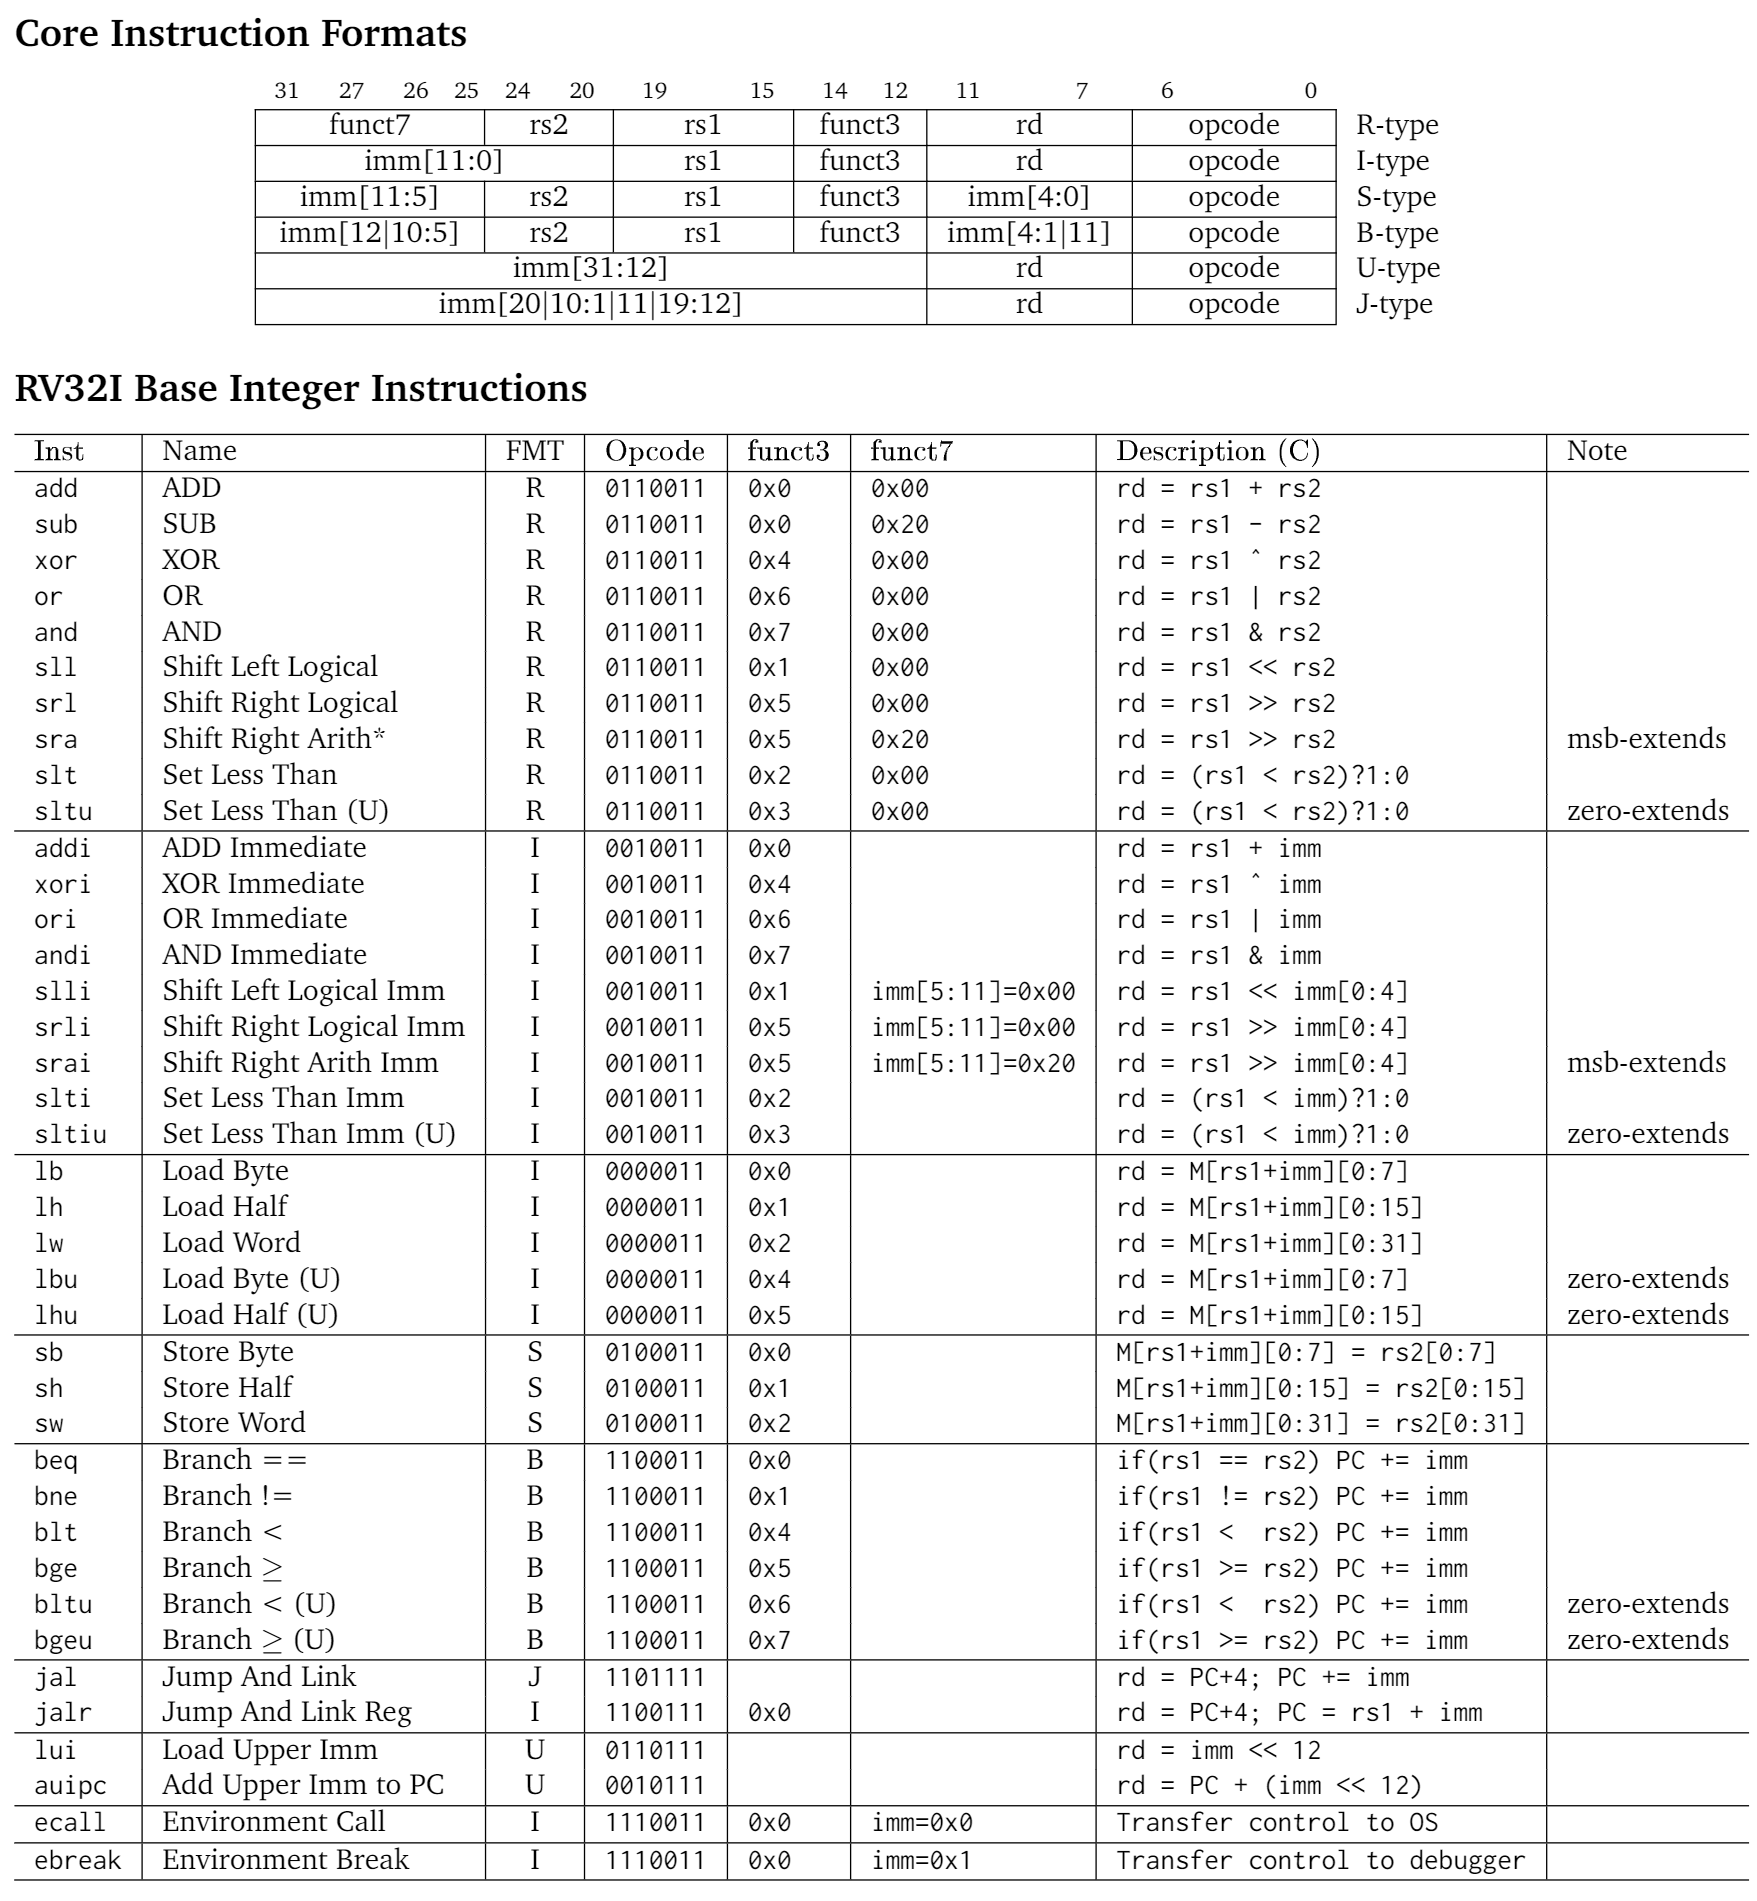
\includegraphics[width=\linewidth]{ISA.png}
    \caption{RV32I指令集索引}
    \label{fig:}
\end{figure}
\subsection{外设模块}
\begin{enumerate}
    \item \textbf{bui模块}
          作为外设的选择模块, 起到了对ram和gpio模块的选择作用, 通过接收mem模块输入的读/写信号及地址信息, 对不同的外设进行读/写操作, 并将需要的读出来的数据返回给mem/wb模块和id模块使用
    \item \textbf{ram模块}
          作为读/写数据的主要存储模块, 是整个CPU的数据“仓库”
    \item \textbf{gpio模块} 同ram模块一样为一组寄存器组, 包含了对十六个按键开关、七段数码管、四个七段数码管选择开关、十六盏LED灯的状态信息, 可以控制上述四类外设是否读取或者写入数据. 
    \item \textbf{rom模块}
          功能为存储各类指令的内容, 出于方便更新指令的考虑, 将rom模块也写成具有读/写功能的模块, 但在正常运行时其写端口信号始终不使能. 
\end{enumerate}
\subsection{编译器}
本项目采用开源的GCC编译器编译C语言程序, 并输入到ROM中, 从而使得CPU的功能设计变得多样化和便利化. 

我们使用的GCC是由eclipse维护的, 使用的版本为xpack-riscv-none-embed-gcc-10.2.0-1.2. 

\subsection{代码风格}

为了保证每个人写的代码可以方便地被所有小组成员阅读,我们详细地制定了
一系列的代码风格规范. 包括
\begin{enumerate}
\item 输入端口在结尾添加\_i标识符,输出端口在结尾添加\_o标识符.
\item 大量使用宏定义,尽量不使用固定的数字,保留对64位架构的可拓展性.
\item 宏定义中,固定的数字全部用大写,不同的单词用下划线隔开;位宽定义用大驼峰命名法.
\item 同一组赋值等号、小括号中括号上下对齐,提高代码的美观性和可读性.
\item 封装常用模块,尽量不直接使用时序always块,减小了代码密度.
\item 所有的命名和注释都严格规范,不允许使用中文作注释.
\item 同一个模块中,严格按照变量声明、时序逻辑块、组合逻辑块、输出逻辑的顺序编写.
\item 全部使用Verilog2001中的端口声明方式. 
\end{enumerate}

\subsection{项目管理}

本次实验全程使用git进行代码管理, 并且将改动实时同步到GitHub上. 本次CPU的代码是完全开源的, 任何人都可以看到我们写的内容, 
甚至为我们提交一些更改. 

项目地址:https://github.com/0xtaruhi/Buceros

\section{CPU各模块实现方式及亮点特色}
\subsection{core\_top核心模块}
\subsubsection{core\_top}
\begin{tabular}{cclll}
    \toprule
    I/O 端口 & 端口类型 & 端口名称      & 端口说明                   & 端口位宽    \\
    \midrule
    input    & wire     & clk           & 时钟信号                   & 1           \\
    input    & wire     & rst\_n        & 异步复位信号(低电平使能) & 1           \\
    input    & wire     & io\_enter     & 流水线恢复信号             & 1           \\

    input    & wire     & inst\_i       & 指令寄存器读指令数据端口   & `WordBus    \\
    input    & wire     & rmem\_data\_i & 内存读数据端口             & `WordBus    \\

    output   & wire     & wmem\_en\_o   & 内存写使能信号             & 1           \\
    output   & wire     & rmem\_en\_o   & 内存读使能信号             & 1           \\
    output   & wire     & wmem\_data\_o & 内存或者gpio写数据端口     & `WordBus    \\
    output   & wire     & rom\_addr\_o  & 指令寄存器读指令地址端口   & `MemAddrBus \\
    output   & wire     & mem\_addr\_o  & 内存访问地址端口           & `MemAddrBus \\
    \bottomrule
\end{tabular}\\
\\
内部集成了流水线的最核心五级, 为与外设相连提供了便利. 

\subsubsection{ctrl}
\begin{tabular}{cclll}
    \toprule
    I/O 端口 & 端口类型 & 端口名称            & 端口说明                      & 端口位宽 \\
    \midrule
    input    & wire     & rst\_n              & 异步复位信号(低电平使能)    & 1        \\
    input    & wire     & stallreq\_id\_ex\_i & 请求暂停信号(来自id/ex模块) & 1        \\
    input    & wire     & enter\_i            & 流水线恢复信号                & 1        \\
    output   & wire     & stall\_o            & 各级流水线暂停端口            & [4:0]    \\
    \bottomrule
\end{tabular}\\
\\若ex中正在执行的命令会影响到id中正在执行的命令, id/ex模块会请求暂停其他级流水线使ex模块的命令优先完成, 并将需要的数据传输回id, 等到传输完毕后id/ex将拉低请求暂停信号, 使流水线继续运转. enter\_i信号从外部输入使流水线重新运行, 消除未知的暂停错误. 
\begin{lstlisting}[language=verilog]
		assign stall_o[0] = stallreq_id_ex_i;   // to pc_reg
		assign stall_o[1] = stallreq_id_ex_i;   // to if_id
		assign stall_o[2] = stallreq_id_ex_i;   // to id_ex
		assign stall_o[3] = 1'b0;               // to ex_mem
		assign stall_o[4] = 1'b0;               // to mem_wb
	\end{lstlisting}
\subsubsection{pc\_reg}
\begin{tabular}{cclll}
    \toprule
    I/O 端口 & 端口类型 & 端口名称     & 端口说明                   & 端口位宽     \\
    \midrule
    input    & wire     & clk          & 时钟信号                   & 1            \\
    input    & wire     & rst\_n       & 异步复位信号(低电平使能) & 1            \\
    input    & wire     & imp\_en\_i   & 跳转命令使能信号           & 1            \\
    input    & wire     & jmp\_addr\_i & 跳转命令地址端口           & `InstAddrBus \\
    input    & wire     & hold\_i      & 暂停命令                   & 1            \\
    output   & reg      & pc\_o        & 命令地址输出端口           & `InstAddrBus \\
    \bottomrule
\end{tabular}\\
\\
此为命令地址计数器, 也为流水线的\textbf{第一级}, 通过对此处的命令地址进行累加或跳转, 从而向rom模块请求不同地址的命令. 
\begin{lstlisting}[language=verilog]
    always @(posedge clk or negedge rst_n) begin
		if(~rst_n) begin
			pc_o <= `PC_RST_ADDR;
        end else if(hold_i) begin
			pc_o <= pc_o;
		end else if(jmp_en_i) begin
			pc_o <= jmp_addr_i;
		end else begin
			pc_o <= pc_o + 32'd4;
		end
	end
\end{lstlisting}
\subsubsection{if\_id}
\begin{tabular}{cclll}
    \toprule
    I/O 端口 & 端口类型 & 端口名称   & 端口说明                   & 端口位宽     \\
    \midrule
    input    & wire     & clk        & 时钟信号                   & 1            \\
    input    & wire     & rst\_n     & 异步复位信号(低电平使能) & 1            \\
    input    & wire     & hold\_i    & 暂停信号                   & 1            \\
    input    & wire     & jmp\_en\_i & 跳转命令使能信号           & 1            \\
    input    & wire     & pc\_i      & 命令地址输入端口           & `InstAddrBus \\
    input    & wire     & inst\_i    & 命令输入端口               & `InstBus     \\
    output   & reg      & pc\_o      & 命令地址输出端口           & `InstAddrBus \\
    output   & reg      & inst\_o    & 命令输出端口               & `InstBus     \\
    \bottomrule
\end{tabular}\\
\\
此为取指/译码寄存器组, 也为流水线的\textbf{第二级}, 将从ROM中提取出来的命令预置在其中, 
并将命令地址一同传递下去. 值得注意的是, 当复位使能或跳转信号使能时, 将inst\_o设置为NOP指令, 
即“addi x0,x0,0”,通过自增0来表示这是一个空指令, 即在跳转指令输入之前先加
载一个空指令以实现立即跳转, 不执行其他指令的功能. 

\subsubsection{id}
\begin{tabular}{cclll}
    \toprule
    I/O 端口 & 端口类型 & 端口名称           & 端口说明                   & 端口位宽     \\
    \midrule
    input    & wire     & rst\_n             & 异步复位信号(低电平使能) & 1            \\
    input    & wire     & pc\_i              & 命令地址输入端口           & `InstAddrBus \\
    input    & wire     & inst\_i            & 命令输入端口               & `InstBus     \\
    input    & wire     & ex\_wreg\_addr\_i  & 执行模块返回数据写地址端口 & `RegAddrBus  \\
    input    & wire     & ex\_wreg\_en\_i    & 执行模块返回数据写使能信号 & 1            \\
    input    & wire     & ex\_wreg\_data\_i  & 执行模块返回数据写数据端口 & `RegDataBus  \\
    input    & wire     & mem\_wreg\_addr\_i & 访存模块返回数据写地址端口 & `RegAddrBus  \\
    input    & wire     & mem\_wreg\_en\_i   & 访存模块返回数据写使能信号 & 1            \\
    input    & wire     & mem\_wreg\_data\_i & 访存模块返回数据写数据端口 & `RegDataBus  \\
    input    & wire     & wb\_wreg\_addr\_i  & 回写模块返回数据写地址端口 & `RegAddrBus  \\
    input    & wire     & wb\_wreg\_en\_i    & 回写模块返回数据写使能信号 & 1            \\
    input    & wire     & wb\_wreg\_data\_i  & 回写模块返回数据写数据端口 & `RegDataBus  \\
    input    & wire     & rs1\_data\_i       & 通用寄存器返回数据一号端口 & `RegDataBus  \\
    input    & wire     & rs2\_data\_i       & 通用寄存器返回数据二号端口 & `RegDataBus  \\
    output   & wire     & branch\_o          & 跳转命令使能信号           & 1            \\
    output   & wire     & pc2pcreg\_o        & 跳转命令地址端口           & `InstAddrBus \\
    output   & wire     & pc2ex\_o           & 命令地址输出端口           & `InstAddrBus \\
    output   & wire     & wmem\_en\_o        & 访存写使能信号             & 1            \\
    output   & wire     & rmem\_en\_o        & 访存读使能信号             & 1            \\
    output   & wire     & opcode\_o          & opcode输出端口             & `OpcodeBus   \\
    output   & wire     & funct3\_o          & funct3输出端口             & `Funct3Bus   \\
    output   & wire     & funct7\_o          & funct7输出端口             & `Funct7Bus   \\
    output   & wire     & imm\_o             & 立即数输出端口             & `ImmBus      \\
    output   & wire     & wreg\_en\_o        & 通用寄存器组写使能信号     & 1            \\
    output   & wire     & wreg\_addr\_o      & 通用寄存器组写使能地址     & `RegAddrBus  \\
    output   & wire     & rs1\_addr\_o       & 通用寄存器组一号地址端口   & `RegAddrBus  \\
    output   & wire     & rs1\_data\_o       & 通用寄存器组一号数据端口   & `RegDataBus  \\
    output   & wire     & rs2\_addr\_o       & 通用寄存器组二号地址端口   & `RegAddrBus  \\
    output   & wire     & rs2\_data\_o       & 通用寄存器组二号数据端口   & `RegDataBus  \\
    \bottomrule
\end{tabular}\\
\\
此模块为五级流水线中\textbf{核心}的译码模块, 其将各类命令割分成各个数据或者地址或者使能信号, 并传递给其他不同的模块\\
\textbf{亮点一}:将从其他模块输入的返回数据写地址端口和信号进行优先级区分, 即ex>mem>wb>regfile, 从而保证当id模块中需要用到的数据正在被ex、mem、wb中的一个操作时能够在最短的时间内将当前数据传回id模块, 尽管使用三级数据比较器增大了延迟, 但保证了电路工作的可靠性\\
\begin{lstlisting}[language=verilog]
assign rs1_data_o  = 
	   (ex_wreg_en_i && ex_wreg_addr_i == rs1_addr_o)  ? ex_wreg_data_i  :
	   (mem_wreg_en_i && mem_wreg_addr_i == rs1_addr_o) ? mem_wreg_data_i :
	   (wb_wreg_en_i && wb_wreg_addr_i == rs1_addr_o)   ? wb_wreg_data_i  :
	   rs1_data_i;
assign rs2_data_o  = 
	   (ex_wreg_en_i && ex_wreg_addr_i == rs2_addr_o)   ? ex_wreg_data_i  :
	   (mem_wreg_en_i && mem_wreg_addr_i == rs2_addr_o) ? mem_wreg_data_i :
	   (wb_wreg_en_i && wb_wreg_addr_i == rs2_addr_o)   ? wb_wreg_data_i  :
	   rs2_data_i;
\end{lstlisting}
\textbf{亮点二}:其他所有的数据选择或者数据分割采用与或选择方式, 大幅度减少了因if、case等逐步选择带来的高延时和高资源使用量. 
\begin{lstlisting}[language=verilog]
//例1
assign branch_o = inst_branch & ( ~funct3_o[2] & ~funct3_o[1] & (funct3_o[0] ^ rs1_eq_rs2) |
funct3_o[2] & ~funct3_o[1] & (funct3_o[0] ^ rs1_lt_rs2) |
funct3_o[2] &  funct3_o[1] & (funct3_o[0] ^ rs1_ltu_rs2)) | inst_jal | inst_jalr;
\end{lstlisting}
\begin{lstlisting}[language=verilog]
//例2
assign imm_o = {`IMM_W{inst_type_I}} & {{20{inst_i[31]}}, inst_i[31:20]} |
	{`IMM_W{inst_type_S}} & {{20{inst_i[31]}}, inst_i[31:25], inst_i[11:7]} |
	{`IMM_W{inst_type_B}} & {{20{inst_i[31]}}, inst_i[7], inst_i[30:25], 
	inst_i[11:8], 1'b0} |{`IMM_W{inst_type_U}} & {{12{inst_i[31]}}, 
	inst_i[31:12]} |{`IMM_W{inst_type_J}} & {{12{inst_i[31]}}, inst_i[19:12],
	 inst_i[20], inst_i[30:21], 1'b0};
\end{lstlisting}
注意:只有我们通用寄存器组一号地址端口的访问地址与ex、mem、wb输出地址相匹配时, id才会提前读取ex、mem、wb这三个端口中的数据
\textbf{亮点三}:我们尽可能地少利用LUT资源,例如我们在译码阶段只使用了一个31bit的比较器
就实现了无符号数比较和有符号数比较.

\begin{lstlisting}[language=verilog]
assign rs_diff_signed = rs1_data_o[`REG_DATA_W-1] ^ rs2_data_o[`REG_DATA_W-1];
assign rs1_ltu_rs2_exclude_msb = rs1_data_o[`REG_DATA_W-2:0] < rs2_data_o[`REG_DATA_W-2:0];
assign rs1_ltu_rs2 = rs_diff_signed ? rs2_data_o[`REG_DATA_W-1] : rs1_ltu_rs2_exclude_msb;
assign rs1_lt_rs2  = rs_diff_signed ? rs1_data_o[`REG_DATA_W-1] : rs1_ltu_rs2_exclude_msb;
\end{lstlisting}

\subsubsection{id\_ex}
\begin{tabular}{cclll}
    \toprule
    I/O 端口 & 端口类型 & 端口名称            & 端口说明                   & 端口位宽     \\
    \midrule
    input    & wire     & clk                 & 时钟信号                   & 1            \\
    input    & wire     & rst\_n              & 异步复位信号(低电平使能) & 1            \\
    input    & wire     & hold\_i             & 暂停信号                   & 1            \\

    input    & wire     & id\_pc\_i           & 命令地址输入端口           & `InstAddrBus \\
    input    & wire     & id\_wmem\_en\_i     & 访存写使能信号             & 1            \\
    input    & wire     & id\_rmem\_en\_i     & 访存读使能信号             & 1            \\
    input    & wire     & id\_opcode\_i       & opcode输入端口             & `OpcodeBus   \\
    input    & wire     & id\_funct3\_i       & funct3输入端口             & `Funct3Bus   \\
    input    & wire     & id\_funct7\_i       & funct7输入端口             & `Funct7Bus   \\
    input    & wire     & id\_imm\_i          & 立即数输入端口             & `ImmBus      \\

    input    & wire     & id\_wreg\_addr\_i   & 通用寄存器数据写地址端口   & `RegAddrBus  \\
    input    & wire     & id\_wreg\_en\_i     & 通用寄存器数据写使能信号   & 1            \\
    input    & wire     & id\_rs1\_data\_i    & 通用寄存器返回数据一号端口 & `RegDataBus  \\
    input    & wire     & id\_rs2\_data\_i    & 通用寄存器返回数据二号端口 & `RegDataBus  \\

    output   & wire     & ex\_pc\_o           & 命令地址输入端口           & `InstAddrBus \\
    output   & wire     & ex\_wmem\_en\_o     & 访存写使能信号             & 1            \\
    output   & wire     & ex\_rmem\_en\_o     & 访存读使能信号             & 1            \\
    output   & wire     & ex\_opcode\_o       & opcode输出端口             & `OpcodeBus   \\
    output   & wire     & ex\_funct3\_o       & funct3输出端口             & `Funct3Bus   \\
    output   & wire     & ex\_funct7\_o       & funct7输出端口             & `Funct7Bus   \\
    output   & wire     & ex\_imm\_o          & 立即数输出端口             & `ImmBus      \\
    output   & wire     & ex\_wreg\_en\_o     & 通用寄存器组写使能信号     & 1            \\
    output   & wire     & ex\_wreg\_addr\_o   & 通用寄存器组写使能地址     & `RegAddrBus  \\
    output   & wire     & rs1\_data\_o        & 通用寄存器组一号数据端口   & `RegDataBus  \\
    output   & wire     & rs2\_data\_o        & 通用寄存器组二号数据端口   & `RegDataBus  \\
    output   & wire     & stallreq\_id\_ex\_o & 暂停请求信号               & 1            \\
    \bottomrule
\end{tabular}\\
\\
本模块为译码/执行模块, 也为流水线的\textbf{第三级}. 本模块为时序电路, 通过统一的时钟控制id信号或端口向ex传递的时序. 
注意:此处stallreq\_id\_ex\_o为暂停请求信号, 每当id模块需要读取内存中数据时, 将会从此处发送请求暂停命令, 以帮助id能够读到最新状态的数据. 
\begin{lstlisting}[language=verilog]
		//例2
always @(posedge clk or negedge rst_n) begin
	if(~rst_n) begin
		stallreq_id_ex_r <= 1'b0;
	end else if(id_rmem_en_i) begin
		stallreq_id_ex_r <= ~stallreq_id_ex_r;
	end else begin
		stallreq_id_ex_r <= 1'b0;
	end
end
	\end{lstlisting}

\subsubsection{ex}
\begin{tabular}{cclll}
    \toprule
    I/O 端口 & 端口类型 & 端口名称      & 端口说明                   & 端口位宽     \\
    \midrule
    input    & wire     & pc\_i         & 命令地址输入端口           & `InstAddrBus \\
    input    & wire     & wmem\_en\_i   & 访存写使能信号             & 1            \\
    input    & wire     & rmem\_en\_i   & 访存读使能信号             & 1            \\
    input    & wire     & opcode\_i     & opcode输入端口             & `OpcodeBus   \\
    input    & wire     & funct3\_i     & funct3输入端口             & `Funct3Bus   \\
    input    & wire     & funct7\_i     & funct7输入端口             & `Funct7Bus   \\
    input    & wire     & imm\_i        & 立即数输入端口             & `ImmBus      \\

    input    & wire     & wreg\_addr\_i & 通用寄存器数据写地址端口   & `RegAddrBus  \\
    input    & wire     & wreg\_en\_i   & 通用寄存器数据写使能信号   & 1            \\
    input    & wire     & rs1\_data\_i  & 通用寄存器返回数据一号端口 & `RegDataBus  \\
    input    & wire     & rs2\_data\_i  & 通用寄存器返回数据二号端口 & `RegDataBus  \\

    output   & wire     & wmem\_en\_o   & 访存写使能信号             & 1            \\
    output   & wire     & rmem\_en\_o   & 访存读使能信号             & 1            \\
    output   & wire     & mem\_addr\_o  & 访存地址端口               & `MemAddrBus  \\
    output   & wire     & funct3\_o     & funct3输出端口             & `Funct3Bus   \\
    output   & wire     & wreg\_en\_o   & 通用寄存器组写使能信号     & 1            \\
    output   & wire     & wreg\_addr\_o & 通用寄存器组写地址端口     & `RegAddrBus  \\
    output   & wire     & wreg\_data\_o & 通用寄存器组写数据端口     & `RegDataBus  \\
    \bottomrule
\end{tabular}\\
\\
本模块为五级流水线中核心的执行模块, 通过对不同指令做对应的基础操作, 从而将计算得到的结果输出到对应的内存中或者转存到通用寄存器组中. 
\textbf{注意一:}经过本次操作后, funct7不再存在利用价值, 而funct3还将决定之后存储到内存中的方式, 包括字节加载、半字加载、字加载、字节加载、半字加载等操作. 
\textbf{注意二:}内存的访问地址由rs1\_data\_i 和 imm\_i 相加得到, 其中rs1\_data\_i 可以由rom中的指令用立即数左移直接加载得到(LUI指令), 而imm\_i可以提前由rom中的指令预置好, 因此, 每一步内存的访问地址都已经由rom中指令决定好了. 
\begin{lstlisting}[language=verilog]
assign mem_addr_o   = rs1_data_i + imm_i;
\end{lstlisting}
\subsubsection{ex\_mem}
\begin{tabular}{cclll}
    \toprule
    I/O 端口 & 端口类型 & 端口名称           & 端口说明                   & 端口位宽    \\
    \midrule
    input    & wire     & clk                & 时钟信号                   & 1           \\
    input    & wire     & rst\_n             & 异步复位信号(低电平使能) & 1           \\
    input    & wire     & hold\_i            & 暂停信号                   & 1           \\

    input    & wire     & ex\_wmem\_en\_i    & 访存写使能信号             & 1           \\
    input    & wire     & ex\_rmem\_en\_i    & 访存读使能信号             & 1           \\
    input    & wire     & ex\_mem\_addr\_i   & 访存地址端口               & `MemAddrBus \\
    input    & wire     & ex\_funct3\_i      & funct3输入端口             & `Funct3Bus  \\
    input    & wire     & ex\_wreg\_addr\_i  & 通用寄存器数据写地址端口   & `RegAddrBus \\
    input    & wire     & ex\_wreg\_en\_i    & 通用寄存器数据写使能信号   & 1           \\
    input    & wire     & ex\_wreg\_data\_i  & 通用寄存器数据写数据端口   & `RegDataBus \\

    output   & wire     & mem\_wmem\_en\_o   & 访存写使能信号             & 1           \\
    output   & wire     & mem\_rmem\_en\_o   & 访存读使能信号             & 1           \\
    output   & wire     & mem\_mem\_addr\_o  & 访存地址端口               & `MemAddrBus \\
    output   & wire     & mem\_funct3\_o     & funct3输出端口             & `Funct3Bus  \\
    output   & wire     & mem\_wreg\_en\_o   & 通用寄存器组写使能信号     & 1           \\
    output   & wire     & mem\_wreg\_addr\_o & 通用寄存器组写地址端口     & `RegAddrBus \\
    output   & wire     & mem\_wreg\_data\_o & 通用寄存器组写数据端口     & `RegDataBus \\
    \bottomrule
\end{tabular}\\
\\
本模块为五级流水线中的ex/mem 模块, 也是流水线中的\textbf{第四级}. 起到了缓存数据, 统一时序的功能. 
\textbf{注意:}各级的寄存器组采用gen\_dffr和gen\_dffsr来模仿D触发器组功能. 
\begin{lstlisting}[language=verilog]
gen_dffr #(.WIDTH(       1'b1)) dff_wmem_en  (clk, rst_n, hold_i, ex_wmem_en_i, mem_wmem_en_o);
gen_dffr #(.WIDTH(       1'b1)) dff_rmem_en  (clk, rst_n, hold_i, ex_rmem_en_i, mem_rmem_en_o);
gen_dffr #(.WIDTH(`MEM_ADDR_W)) dff_mem_addr (clk, rst_n, hold_i, ex_mem_addr_i, mem_mem_addr_o);
gen_dffr #(.WIDTH(  `FUNCT3_W)) dff_funct3   (clk, rst_n, hold_i, ex_funct3_i, mem_funct3_o);
gen_dffr #(.WIDTH(       1'b1)) dff_wreg_en  (clk, rst_n, hold_i, ex_wreg_en_i, mem_wreg_en_o);
gen_dffr #(.WIDTH(`REG_ADDR_W)) dff_wreg_addr(clk, rst_n, hold_i, ex_wreg_addr_i, mem_wreg_addr_o);
gen_dffr #(.WIDTH(`REG_DATA_W)) dff_wreg_data(clk, rst_n, hold_i, ex_wreg_data_i, mem_wreg_data_o);
\end{lstlisting}
\subsubsection{mem}
\begin{tabular}{cclll}
    \toprule
    I/O 端口 & 端口类型 & 端口名称      & 端口说明                      & 端口位宽    \\
    \midrule
    input    & wire     & wmem\_en\_i   & 访存写使能信号                & 1           \\
    input    & wire     & rmem\_en\_i   & 访存读使能信号                & 1           \\
    input    & wire     & mem\_addr\_i  & 访存地址端口                  & `MemAddrBus \\
    input    & wire     & rmem\_data\_i & 来自内存的读取数据端口        & `MemDataBus \\
    input    & wire     & funct3\_i     & funct3输入端口                & `Funct3Bus  \\
    input    & wire     & wreg\_addr\_i & 通用寄存器数据写地址端口      & `RegAddrBus \\
    input    & wire     & wreg\_en\_i   & 通用寄存器数据写使能信号      & 1           \\
    input    & wire     & wreg\_data\_i & 通用寄存器/内存数据写数据端口 & `RegDataBus \\

    output   & wire     & wmem\_en\_o   & 访存写使能信号                & 1           \\
    output   & wire     & rmem\_en\_o   & 访存读使能信号                & 1           \\
    output   & wire     & mem\_addr\_o  & 访存地址端口                  & `MemAddrBus \\
    output   & wire     & wmem\_data\_o & 写内存数据端口                & `WordBus    \\
    output   & wire     & wreg\_en\_o   & 通用寄存器组写使能信号        & 1           \\
    output   & wire     & wreg\_addr\_o & 通用寄存器组写地址端口        & `RegAddrBus \\
    output   & wire     & wreg\_data\_o & 通用寄存器组写数据端口        & `RegDataBus \\
    \bottomrule
\end{tabular}\\
\\
本模块为五级流水线中的核心模块, 即访存模块. wreg\_data\_o既可以输入到通用寄存器组中, 也可以输入到内存当中, 其选择由各个使能信号决定. 而wreg\_data\_o与wmem\_data\_o由wreg\_data\_i根据funct3\_i与使能信号选择性加载得到, 实现了指令的功能. 
注意:此处对写入的数据进行字节加载、半字加载、字加载、字节加载、半字加载等操作. 
\begin{lstlisting}[language=verilog]
always @ (*) begin
	if (wmem_en_i) begin
		case (funct3_i)
			`INST_BYTE: begin
				wmem_data_r = {{(`ROM_WIDTH - `BYTE_WIDTH){1'b0}},wreg_data_i[`BYTE_WIDTH - 1:0]};
			end
			`INST_HALF_WORD: begin
				wmem_data_r = {{(`ROM_WIDTH - `HALF_WORD_WIDTH){1'b0}},wreg_data_i[`HALF_WORD_WIDTH - 1:0]};
			end
			`INST_WORD: begin
				wmem_data_r = wreg_data_i; // not extended to ARCH_RV64, so the code has been simplified
			end
			default: begin
				wmem_data_r = `ZERO_WORD;
			end
		endcase
		wreg_data_r = `ZERO_WORD; // when store, do nothing with wreg_data
	end else if (rmem_en_i) begin
		wmem_data_r = `ZERO_WORD;
		case (funct3_i)
			`INST_BYTE: begin
				wreg_data_r = {{(`ROM_WIDTH - `BYTE_WIDTH){rmem_data_i[`BYTE_WIDTH - 1]}},rmem_data_i[`BYTE_WIDTH - 1:0]};
			end
			`INST_HALF_WORD: begin
				wreg_data_r = {{(`ROM_WIDTH - `HALF_WORD_WIDTH){rmem_data_i[`HALF_WORD_WIDTH - 1]}},rmem_data_i[`HALF_WORD_WIDTH - 1]};
			end
			`INST_WORD: begin
				wreg_data_r = rmem_data_i; // not extended to ARCH_RV64, so the code has been simplified
			end
			`INST_BYTE_U: begin
				wreg_data_r = {{(`ROM_WIDTH - `BYTE_WIDTH){1'b0}},rmem_data_i[`BYTE_WIDTH - 1:0]};
			end
			`INST_HALF_WORD_U: begin
				wreg_data_r = {{(`ROM_WIDTH - `HALF_WORD_WIDTH){1'b0}},rmem_data_i[`HALF_WORD_WIDTH - 1]};
			end
			default: begin
				wreg_data_r = `ZERO_WORD;
			end
			endcase
		end else begin
			wmem_data_r = `ZERO_WORD;
			wreg_data_r = wreg_data_i;
		end
	end
\end{lstlisting}
\subsubsection{mem\_wb}
\begin{tabular}{cclll}
    \toprule
    I/O 端口 & 端口类型 & 端口名称           & 端口说明                   & 端口位宽    \\
    \midrule
    input    & wire     & clk                & 时钟信号                   & 1           \\
    input    & wire     & rst\_n             & 异步复位信号(低电平使能) & 1           \\
    input    & wire     & hold\_i            & 暂停信号                   & 1           \\

    input    & wire     & mem\_wreg\_addr\_i & 通用寄存器数据写地址端口   & `RegAddrBus \\
    input    & wire     & mem\_wreg\_en\_i   & 通用寄存器数据写使能信号   & 1           \\
    input    & wire     & mem\_wreg\_data\_i & 通用寄存器写数据端口       & `RegDataBus \\

    output   & wire     & wb\_wreg\_en\_o    & 通用寄存器组写使能信号     & 1           \\
    output   & wire     & wb\_wreg\_addr\_o  & 通用寄存器组写地址端口     & `RegAddrBus \\
    output   & wire     & wb\_wreg\_data\_o  & 通用寄存器组写数据端口     & `RegDataBus \\
    \bottomrule
\end{tabular}\\
\\
本模块为五级流水线中的mem\_wb模块, 也是流水线的\textbf{最后一级}. 其作为通用寄存器组, 输出既可以发送到regfile并写入数据和地址, 也可以发送到id模块直接提供数据和地址. 使得整个流水线成为一个可反馈的循环网络. 

\subsubsection{regfile}
\begin{tabular}{cclll}
    \toprule
    I/O 端口 & 端口类型 & 端口名称    & 端口说明                   & 端口位宽    \\
    \midrule
    input    & wire     & clk         & 时钟信号                   & 1           \\
    input    & wire     & rst\_n      & 异步复位信号(低电平使能) & 1           \\

    input    & wire     & r\_addr1\_i & 通用寄存器返回地址一号端口 & `RegAddrBus \\
    input    & wire     & r\_addr2\_i & 通用寄存器返回地址二号端口 & `RegAddrBus \\
    input    & wire     & w\_en\_i    & 通用寄存器写使能信号       & 1           \\
    input    & wire     & w\_addr\_i  & 通用寄存器写地址端口       & `RegAddrBus \\
    input    & wire     & w\_data\_i  & 通用寄存器写数据端口       & `RegDataBus \\


    output   & wire     & r\_data1\_o & 通用寄存器输出数据一号端口 & `RegDataBus \\
    output   & wire     & r\_data2\_o & 通用寄存器输出数据二号端口 & `RegDataBus \\
    \bottomrule
\end{tabular}\\
\\
本模块为五级流水线的数据“数据中转站”\_\_通用寄存器组. 在此处加载诸多临时存放的数据, 以供id模块使用. 共有32个字长为32位的通用寄存器(x0~x31), 其中x0寄存器中数据恒为0. 对于数据的读取部分, 采用组合逻辑描述, 在最短的时间内读取到对应寄存器的数据. 对于数据的写入部分, 采用同步时序电路描述, 类似于rom、ram、gpio的操作. 具体的用途可见下页图3. 

\begin{lstlisting}[language=verilog]
assign r_data1_o = {`REG_DATA_W{~r1_x0}} & ((w_en_i && (r_addr1_i == w_addr_i))
 ? w_data_i : regfile[r_addr1_i]);
assign r_data2_o = {`REG_DATA_W{~r2_x0}} & ((w_en_i && (r_addr2_i == w_addr_i))
 ? w_data_i : regfile[r_addr2_i]);

\end{lstlisting}
% \begin{figure}
%     \centering
%     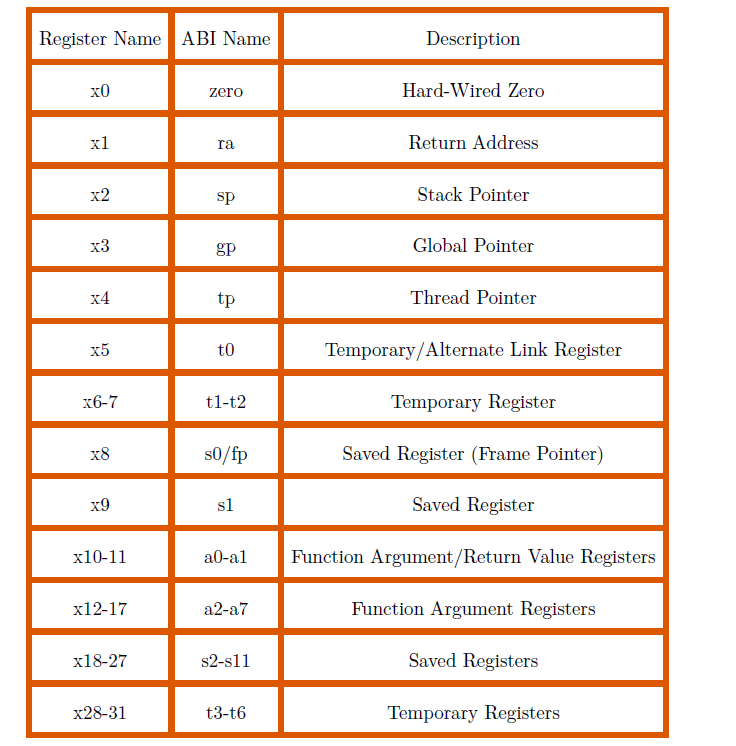
\includegraphics[width=0.7\linewidth]{1640076105(1)}
%     \caption{通用寄存器各部分用途}
%     \label{fig:16400761051}
% \end{figure}
\begin{table}
    \centering
\begin{tabular}{llll}
    \toprule
    寄存器编号 & 寄存器别名 & 描述              & 保存者   \\
    \midrule
    x0         & zero       & 硬编码0           & /        \\
    x1         & ra         & 返回地址          & 调用者   \\
    x2         & sp         & 栈指针            & 被调用者 \\
    x3         & gp         & 全局指针          & /        \\
    x4         & tp         & 线程指针          & /        \\
    x5-7       & t0-2       & 临时变量          & 调用者   \\
    x8         & s0/sp      & 保存寄存器/栈指针 & 被调用者 \\
    x9         & s1         & 保存寄存器        & 被调用者 \\
    x10-11     & a0-1       & 函数入参/返回值   & 调用者   \\
    x12-17     & a2-7       & 函数入参          & 调用者   \\
    x18-27     & s2-11      & 保存寄存器        & 被调用者 \\
    x28-31     & t3-6       & 临时变量          & 调用者   \\
    \bottomrule
\end{tabular}
\caption{通用寄存器相关描述}
\end{table}

\subsubsection{gen\_dffr / gen\_dffsr }
\begin{tabular}{cclll}
    \toprule
    I/O 端口 & 端口类型 & 端口名称 & 端口说明                   & 端口位宽     \\
    \midrule
    input    & wire     & clk      & 时钟信号                   & 1            \\
    input    & wire     & rst\_n   & 异步复位信号(低电平使能) & 1            \\
    input    & wire     & hold\_i  & 暂停信号                   & 1            \\
    input    & wire     & data\_i  & 输入数据端口               & [WIDTH\_1:0] \\

    output   & wire     & data\_o  & 输出数据端口               & [WIDTH\_1:0] \\
    \bottomrule
\end{tabular}\\
\\
本模块为util(工具)类模块, 在此处起到类D触发器的功能. 
\subsection{外设模块}
\subsubsection{biu}
\begin{tabular}{cclll}
    \toprule
    I/O 端口 & 端口类型 & 端口名称      & 端口说明             & 端口位宽    \\
    \midrule
    input    & wire     & mem\_addr\_i  & 内存访问地址端口     & `MemAddrBus \\
    input    & wire     & wmem\_data\_i & 内存写数据输入端口   & `WordBus    \\
    input    & wire     & ram\_data\_i  & ram读取数据输入端口  & `MemDataBus \\
    input    & wire     & gpio\_data\_i & gpio读取数据输入端口 & `MemDataBus \\

    output   & wire     & gpio\_en\_o   & gpio选择使能信号     & 1           \\
    output   & wire     & rmem\_data\_o & 内存读数据输出端口   & `MemDataBus \\
    \bottomrule
\end{tabular}\\
\\
本模块是外设模块中的\textbf{核心biu模块}, 为组合逻辑电路, 该模块可以对外设(ram, gpio)起到选择作用.根据输入的内存访问地址端口, 可以使ram\_en\_o或者gpio\_en\_o使能, 选择对应的外设. \textbf{写操作:}写数据及写地址都已经由mem提供到各个外设模块. \textbf{读操作:}对应的选择信号使能后, 将对应的外设输入的读数据通过biu输出回core\_top模块. 

\subsubsection{gpio}
\begin{tabular}{cclll}
    \toprule
    I/O 端口 & 端口类型 & 端口名称         & 端口说明                   & 端口位宽    \\
    \midrule
    input    & wire     & clk              & 时钟信号                   & 1           \\
    input    & wire     & rst\_n           & 异步复位信号(低电平使能) & 1           \\
    input    & wire     & en\_i            & 使能选择信号               & 1           \\

    input    & wire     & r\_en\_i         & 读使能信号                 & 1           \\
    input    & wire     & addr\_i          & 访问地址输入端口           & `MemAddrBus \\
    input    & wire     & w\_en\_i         & 写使能信号                 & 1           \\
    input    & wire     & w\_data\_i       & 写数据输入端口             & `MemDataBus \\
    input    & wire     & pin\_sw\_i       & 外部输入开关信号           & [15:0]      \\

    output   & wire     & r\_data\_o       & 读数据输出端口             & `MemDataBus \\
    output   & wire     & pin\_seg\_o      & 七段数码管显示输出端口     & 7:0         \\
    output   & wire     & pin\_seg\_sel\_o & 七段数码管选通输出端口     & 3:0         \\
    output   & wire     & pin\_led\_o      & 流水灯显示输出端口         & 15:0        \\
    \bottomrule
\end{tabular}\\
\\
本模块为外设部分中的\textbf{GPIO}(General\_purpose input/output)模块, 其中, 按键开关信息由外部直接读入, 无法写入, 但七段数码管的显示、选通以及流水灯可以实现写入和读取. 选择不同的外设, 从而使得能够将计算的结果输出显示. 

\subsubsection{ram}
\begin{tabular}{cclll}
    \toprule
    I/O 端口 & 端口类型 & 端口名称   & 端口说明                   & 端口位宽    \\
    \midrule
    input    & wire     & clk        & 时钟信号                   & 1           \\
    input    & wire     & rst\_n     & 异步复位信号(低电平使能) & 1           \\

    input    & wire     & addr\_i    & 访问地址输入端口           & `MemAddrBus \\
    input    & wire     & w\_en\_i   & 写使能信号                 & 1           \\
    input    & wire     & w\_data\_i & 写数据输入端口             & `WordBus    \\
    input    & wire     & w\_sel\_i  & 字节选择信号               & [3:0]       \\

    output   & wire     & r\_data\_o & 读数据输出端口             & `WordBus    \\
    \bottomrule
\end{tabular}\\
\\
此为外设部分中的\textbf{ram}模块, 每一次读写操作对四个字节(即一个字)去操作. 
亮点:可对一个字中的任意几个字节进行写操作, 从而实现对内存中单个或多个字节的修改, 但同时读取时以字为单位进行读取. 

\subsubsection{rom}
\begin{tabular}{cclll}
    \toprule
    I/O 端口 & 端口类型 & 端口名称   & 端口说明                   & 端口位宽    \\
    \midrule
    input    & wire     & clk        & 时钟信号                   & 1           \\
    input    & wire     & rst\_n     & 异步复位信号(低电平使能) & 1           \\

    input    & wire     & r\_addr\_i & 访问地址输入端口           & `MemAddrBus \\
    input    & wire     & w\_en\_i   & 写使能信号                 & 1           \\
    input    & wire     & w\_addr\_i & 访问地址输入端口           & `MemAddrBus \\
    input    & wire     & w\_data\_i & 写数据输入端口             & `WordBus    \\
    input    & wire     & w\_sel\_i  & 字节选择信号               & [3:0]       \\

    output   & wire     & r\_data\_o & 读数据输出端口             & `WordBus    \\
    \bottomrule
\end{tabular}\\
\\
此为外设部分中的\textbf{rom}模块, 每一次读写操作对四个字节(即一个字)去操作. 
注意:此处关于rom的所有写端口在正常工作时全部置于低电平, 内部存储的为指令信息,  借助
\begin{lstlisting}[language=verilog]
initial begin
$readmemh("E:/honorwork/CPU/Buceros/tests/examples/led.mem", _rom);
end
\end{lstlisting}
代码读入对应的汇编代码. 

\subsubsection{地址分配}
\begin{table}[h!]
    \centering
    \begin{tabular}{cclll}
        \toprule
        可用地址空间                           & 实际占用地址空间                       & 设备                 & 类型  & 容量  \\
        \midrule
        \texttt{0x0000\_0000 --- 0x1fff\_ffff} & \texttt{0x0000\_0000 --- 0x0000\_07ff} & 指令存储器(ROM)      & 只读* & 1KB  \\
        \texttt{0x2000\_0000 --- 0x3fff\_ffff} & \texttt{0x2000\_0000 --- 0x2000\_07ff} & 数据存储器(RAM)      & 读/写 & 1KB  \\
        \texttt{0x4000\_0000 --- 0x5fff\_ffff} & \texttt{0x4000\_0000 --- 0x4000\_0001} & GPIO(LED)            & 读/写 & 2Byte \\
        \texttt{0x4000\_0000 --- 0x5fff\_ffff} & \texttt{0x4000\_0004 --- 0x4000\_0005} & GPIO(七段数码管显示) & 读/写 & 2Byte \\
        \texttt{0x4000\_0000 --- 0x5fff\_ffff} & \texttt{0x4000\_0008 --- 0x4000\_0008} & GPIO(七段数码管选通) & 读/写 & 1Byte \\
        \texttt{0x4000\_0000 --- 0x5fff\_ffff} & \texttt{0x5000\_0000 --- 0x5000\_0001} & GPIO(开关)           & 只读  & 2Byte \\
        \bottomrule
    \end{tabular}
\end{table}
\section{编译器}

\subsection{Makefile文件}

我们利用了make这一工具进行编译. 编译完成后会产生.bin .dump .mem .o 四个文件.


\subsection{链接文件}

链接文件中指定了程序各个部分所在的位置. 在链接文件的一开头就有如下两句:

\begin{lstlisting}
MEMORY
{
    rom(wxa!ri) : ORIGIN = 0x00000000, LENGTH = 1K
    ram(wxa!ri) : ORIGIN = 0x20000000, LENGTH = 1K
}
\end{lstlisting}
这就指明了程序可用的rom和ram空间. 我们采用的是哈佛结构(在RISCV/ARM嵌入式结构中非常常见),
随后即是各个section位置的说明. 特别要说明的是“栈空间”,在lds文件中时这么描述的:
\begin{lstlisting}
.stack ORIGIN(ram) + LENGTH(ram) - __stack_size :
{
    PROVIDE( _heap_end = . );
    . = __stack_size;
    PROVIDE( _sp = . );
    __freertos_irq_stack_top = .;
} >ram AT>ram
\end{lstlisting}

栈是负增长的,所以需要把初始栈指针\_sp设置在栈顶. 在入口汇编程序中需要用到这个值. 

\begin{lstlisting}]
    la sp, _sp
\end{lstlisting}
\subsection{从bin转到mem}

由于编译出来的文件是bin格式的二进制文件,我们使用了Python程序将bin转换为mem. 

程序如下\lstinputlisting[language=python]{../tests/bin2mem.py}

\subsection{编译}

编译非常简单,在配置好环境之后,cd到程序所在的文件夹(必须有Makefile文件),然后输入
\begin{lstlisting}[language=bash]
make
\end{lstlisting}
就会自动在文件夹里生成一个mem文件.
\section{测试实验}

\section{我们解决的一些bug}

\subsection{BUG1——运算符优先级}
错误代码
\begin{lstlisting}[language=verilog]
assign result_sum   = rs1_data_i + (exe_sub ^ data2 + exe_sub);
\end{lstlisting}

正确代码
\begin{lstlisting}[language=verilog]
assign result_sum   = rs1_data_i + (({`REG_DATA_W{exe_sub}} ^ data2) + exe_sub);
\end{lstlisting}

\subsection{BUG2——流水线吞指令}
错误代码
\begin{lstlisting}[language=verilog]
assign stall_o[0] = stallreq_id_ex_i;   // to pc_reg
assign stall_o[1] = stallreq_id_ex_i;   // to if_id
assign stall_o[2] = stallreq_id_ex_i;   // to id_ex
assign stall_o[3] = 1'b0;               // to ex_mem
assign stall_o[4] = stallreq_id_ex_i;
\end{lstlisting}

正确代码
\begin{lstlisting}[language=verilog]
assign stall_o[0] = stallreq_id_ex_i;   // to pc_reg
assign stall_o[1] = stallreq_id_ex_i;   // to if_id
assign stall_o[2] = stallreq_id_ex_i;   // to id_ex
assign stall_o[3] = 1'b0;               // to ex_mem
assign stall_o[4] = 1'b0;
\end{lstlisting}

\subsection{BUG3——PC寄存器的hold与jump}

错误代码
\begin{lstlisting}[language=verilog]
always @(posedge clk or negedge rst_n) begin
    if(~rst_n) begin
        pc_o <= `PC_RST_ADDR;
    end else if(jmp_en_i) begin
        pc_o <= jmp_addr_i;
    end else if(hold_i) begin
        pc_o <= pc_o;
    end else begin
        pc_o <= pc_o + 32'd4;
    end
end
\end{lstlisting}

正确代码
\begin{lstlisting}[language=verilog]
always @(posedge clk or negedge rst_n) begin
    if(~rst_n) begin
        pc_o <= `PC_RST_ADDR;
    end else if(hold_i) begin
        pc_o <= pc_o;
    end else if(jmp_en_i) begin
        pc_o <= jmp_addr_i;
    end else begin
        pc_o <= pc_o + 32'd4;
    end
end
\end{lstlisting}

\section{一些问题和自己的思考}

\subsection{为什么我们不做VGA显示?}

VGA显示需要使用自己的频率. 一方面我们不希望把VGA模块用Verilog写死,
而是希望通过程序的方式进行实现,否则就违背了做一个“CPU”的初衷,之后
在调节主频的时候也会出现问题. 我们希望CPU的频率是灵活可调节的.

\section{不足及总结}

\subsection{架构设计失误}

我们将所有的读取做成了组合逻辑,后续证明我们的频率之所以上不去,
就是因为mem的读取延迟过大. 我们当时应该采用时序逻辑的做法,
这样可以显著地减少建立时间,大大提高我们CPU的主频.

同时将ram和rom做成时序逻辑还可以调用板上的bram资源. 我们当时开始时
预想的ram和rom各有64K的大小,但是最后只实现了各1K的大小. 一方面,由于不能
使用bram资源,所有的存储都是用lut资源实现的,这使得综合非常缓慢. 另一方面,
及时只有1K的大小,也占用了18\%的lut资源,相比之下我们的cpu只用了4\%的lut资源.

\end{document}